\section{Object Detection with Convolutional Neural Networks}\label{sec:objdet}
This section will perform a technical analysis of some of the current leading \gls{cnn}-based object detectors. This includes Faster R-CNN \cite{fasterrcnn}, \gls{rfcn} \cite{rfcn} and YOLOv2 \cite{yolov2}. On top of the analysis, results for the detectors will be discussed for \gls{pascalvoc} and \gls{mscoco}. This should given an indication as to which \gls{cnn}-based object detector will be used to address robustness-related challenges. Additionally, two common choices for backbones models will be explained.

\subsection{Faster Region-Convolutional Neural Network}
A primary \gls{cnn}-based object detector over the previous years has been Faster R-CNN \cite{fasterrcnn} and its predecessors, Fast R-CNN \cite{fastrcnn} and R-CNN \cite{rcnn}. As mentioned in \sectionref{related}, 15 of the 21 current entries in \gls{mscoco} are Faster R-CNN based. The general method of Faster R-CNN can be split into two parts, region proposals and region classification. Region proposals aims to reduce the amount of windows that need to be tested at inference time in comparison to the previously often used sliding window approach. Rather than testing a plethora of potential object window locations, scales and aspect ratios, region proposals find a lower number of windows that are likely to contain an object. Additionally, it also allows for using more expensive classification techniques such as \glspl{cnn}. There are a large number of different methods to compute region proposals. However, the \gls{rpn} in Faster R-CNN is one of the more popular and is used in other \gls{cnn}-based approaches. The proposals are efficiently computed with the \gls{rpn}, as proposals are found directly in the network, sharing convolutional layers with the classification step. The framework of the Faster R-CNN can be seen in \figref{fasterframework}, where the convolutional layers are used to compute feature maps. On the last feature map, the \gls{rpn} computes region proposals. These are then placed back onto the last feature map and \gls{roi} pooling is used to compute features for classification.

\begin{figure}[H]
  \centering
    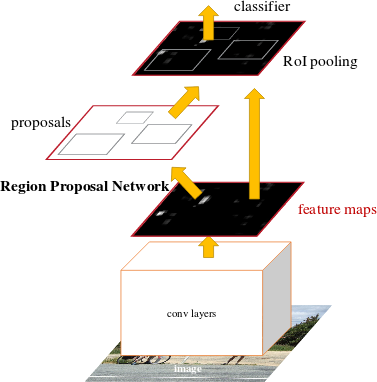
\includegraphics[width=0.6\textwidth]{Figs/Techanal/fasterframework.png}
      \caption{Faster R-CNN framework. A \gls{cnn} computes a feature map from which a \gls{rpn} finds region proposals. Given these proposals and the same feature map proposals are classed accordingly \cite{fasterrccn}.}
    \label{fig:fasterframework}
\end{figure}

There are a number of different possible \gls{cnn} models that can be used the compute feature maps through the convolutional layers. In the original Faster R-CNN VGG nets \cite{vgg16} were experimented with. However, since then more efficient and accurate networks have come forward, with one of the most popular being the ResNet \cite{deepres} architecture. Both of the models will be covered in more depth later in this chapter. Standard practice is to pre-train the network for classification on ImageNet followed by fine-tuning it towards object detection. Independent of the chosen network the \gls{rpn} takes as input the last feature map from the convolutional layers of the network. A small network traverses the feature map which feeds the result into two sibling fully-connected layers, a box-classification layer and a box regression layer. The box-classification layer classifies the \gls{roi} into either an object or background, with a probability being associated to each. While the box-regression layer attempts to fit the bounding-box to the object of interest. In order to take into account different scales and aspect ratios of objects in the feature map, the \gls{rpn} uses a set of pre-defined \glspl{roi} at each sliding window location. These pre-defined \glspl{roi} are denoted as anchors. At each sliding window location a maximum of $k$ possible region proposals can be computed based upon the $k$ anchors. The anchors are user-defined into different sizes and aspect ratios. An often used default setting for the anchors is $k$ = 9, which corresponds to all combinations of 3 scales and 3 aspect ratios. The computation of the $k$ anchors at a sliding window location followed by the sibling layers is visualised in \figref{rpnframework}.

\begin{figure}[H]
  \centering
    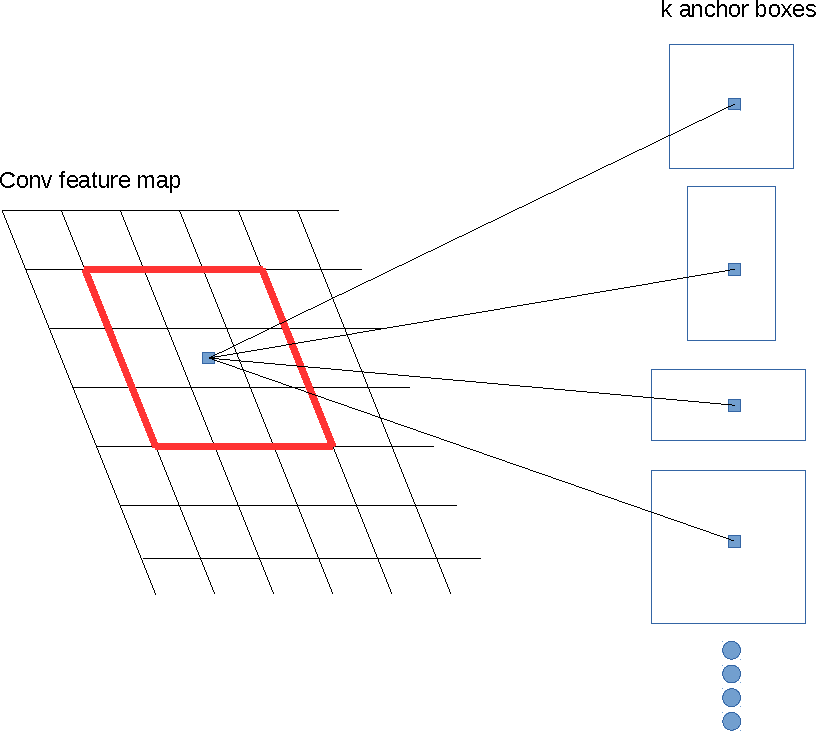
\includegraphics[width=0.6\textwidth]{Figs/Techanal/rpn1-crop.pdf}
      \caption{\gls{rpn} framework. The $k$ anchor boxes are placed at each sliding window location on the last feature map. The \gls{rpn} uses two sibling layers to compute the classification of object or background and perform bounding-box regression.}
    \label{fig:rpnframework}
\end{figure}

Given the set of region proposals from the \gls{rpn}, objects are classified in the $C+1$ categories based upon the same approach as in Fast R-CNN. Where $C$ are the total number of object classes plus one background class. Features are cropped for each proposal are their respective location from the same feature map given to the \gls{rpn}. Features are computed using a \gls{roi} pooling layer that uses max pooling to convert the cropped area into a pooled map of fixed spatial extent ($H \times W$), where $H$ and $W$ are hyper-parameters. In order convert each \gls{roi} into a fixed max pooled size, the \gls{roi} of size $h \times w$ is split into a grid of $H \times W$, with each sub-window being of size $h/H \times w/W$. Max pooling is then applied at each sub-window and placed accordingly in the $H \times W$ pooled layer. Following the \gls{roi} pooling layer, two fully-connected layers feed sibling layers into a classification layer and a box-regression layer, similar to those in the \gls{rpn}. However, in this instance the classification layer computes the probabilities for each of the $C+1$ classes.

\subsection{Region-Based Fully-Connected Network}
One of the current leading object detection methods is the \gls{rfcn} \cite{rfcn}, which as mentioned in \sectionref{related}, takes a different approach to that of the region-based methods such as Faster R-CNN. The authors of \gls{rfcn} were inspired by the recent advances in \gls{fcn} classification networks, such as ResNets, and argue that the addition of the \gls{roi}-pooling layer in the Faster R-CNN pipeline is unnatural and adds computational complexity. The authors hypothesise that the reasoning behind this addition is due to the trade-off between using a classification approach in an object detection pipeline. A defining factor in object detection is that the method should be able to respect translation variance, that translation of an object inside an object proposal should given a good indication as to how well the proposal fits the object. Whereas classification is more translation invariant, as the shifting of an object in an image does not effect how the system returns it's output. The use of the \gls{roi}-pooling layer placed in between convolutional layers means that any convolutions after this point are not translation invariant as it is not region specific. Rather than using this popular feature extractor, \gls{rfcn} uses position-sensitive score maps computed by a bank of convolutional layers. The maps add translation variance into the detection pipeline by computing scores in relation to position information with respect to the relative spatial position of an object. A \gls{roi}-pooling layer is added after the score-maps, however, no convolutional operations are done after this point ensuring translation variance.
\\\\
The overall approach of the \gls{rfcn} also consists of the popular two-stages of region proposal and region classification. Region proposal is done using the \gls{rpn} from Faster R-CNN followed by the position-sensitive score maps and \gls{roi} pooling for region classification. The overall architecture of the \gls{rfcn} can be seen in \figref{rfcnarch}. Similar to Faster R-CNN, convolutional layers are applied on the input image and the \gls{rpn} computes region proposals. After this position-sensitive score maps aid in classification.


\begin{figure}[H]
  \centering
    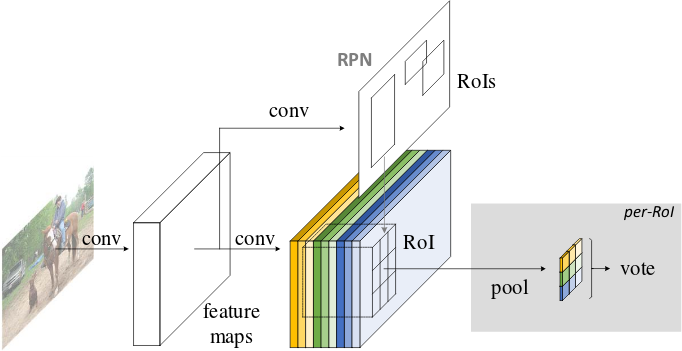
\includegraphics[width=0.8\textwidth]{Figs/Techanal/rfcnarchi.png}
      \caption{Architecture of \gls{rfcn}. Region proposals are found using the \gls{rpn} followed by classification based on a bank of position-sensitive score maps \cite{rfcn}.}
    \label{fig:rfcnarch}
\end{figure}

The added translation variance post finding proposals with the \gls{rpn} is done by producing a bank of $k^2$ score maps for each object category. Therefore, there are a total of $k^2(C + 1)$ maps. The number of $k^2$ maps is due to a $k \times k$ spatial grid representing relative positions. Typically $k = 3$, therefore, nine score maps represent position-sensitive scores for a given object category. This is illustrated in \figref{scoremaps}, each of the 9 coloured rectangles on the left of the figure represent the $k^2$ score maps. Each colour represents one of the relative positions. For example, the three shades of blue are positions in the bottom of a \gls{roi}, where the darkest is bottom-right, then bottom-centre and lightest bottom-right. For a given \gls{roi} placement the vote for relative position is sampled from their respective map in the bank.

\begin{figure}[H]
  \centering
    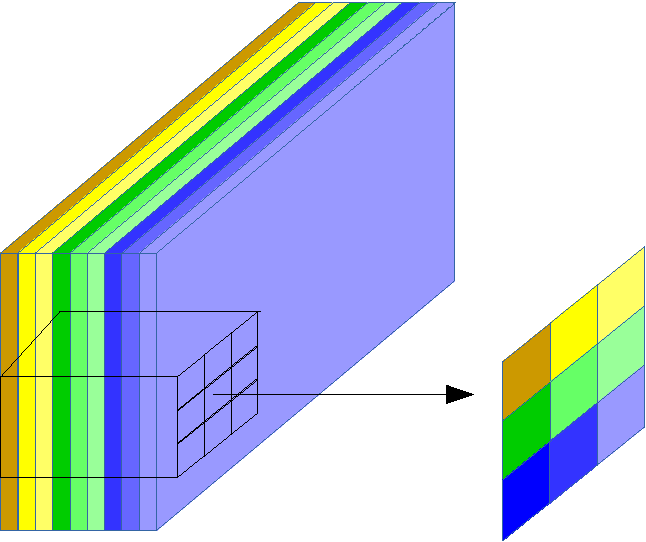
\includegraphics[width=0.4\textwidth]{Figs/Techanal/scoremaps-crop.pdf}
     \caption{A bank of score maps are present for each object category. For a given \gls{roi}, the score is sampled from the respective position in the corresponding score map.}
    \label{fig:scoremaps}
\end{figure}

Once the bank of score maps have been computed, position-sensitive \gls{roi}-pooling is found for region classification. Each individual $k \times k$ bin pools from its corresponding location in the relevant score map. For example, the top left bin pools from that position in the top-left score map and so on. The \gls{roi}-pool is computed using average pooling for each bin which can be seen in \figref{rfcnpooling}. The final decision for a given class is determined by a vote where each of the bins are averaged, producing a $(C+1)$-dimensional vector for each \gls{roi}.

\begin{figure}[H]
  \centering
    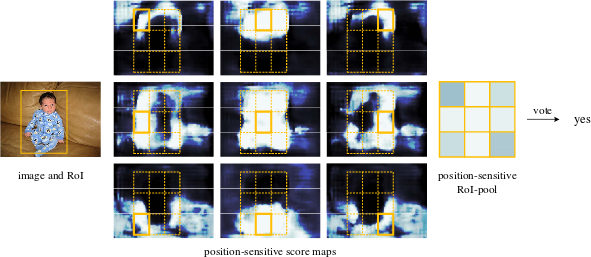
\includegraphics[width=1.0\textwidth]{Figs/Techanal/rfcnpooling.png}
      \caption{Position-sensitive \gls{roi}-pooling operation for a given class \cite{rfcn}.}
    \label{fig:rfcnpooling}
\end{figure}

\subsection{You Only Look Once}
YOLOv2 \cite{yolov2} is one of the current best performing single shot detectors, with results on par with more commonly used object detectors while being considerably faster at test time. YOLOv2 uses a different approach than the common 2-step method of region proposal and region classification seen in Faster R-CNN and \gls{rfcn} by directly computing class probabilities on each \gls{roi}. Some of the distinct difference between YOLOv2 and region-based methods is the use of directly predicting bounding boxes, using a modified model, and altering how the priors for anchor boxes are computed during region proposals with the \gls{rpn}. The distinct differentiator for YOLO and YOLOv2 is that bounding boxes for a given object are predicted directly rather than predicting offsets to anchors with the \gls{rpn}. This is done by splitting the image into $S \times S$ grid cells, with each cell predicting $B$ bounding boxes. Each of the $B$ boxes predict a total of 5 values: $[t_x, t_y, t_w, t_h, t_o]$. Where $t_x, t_y$ are the coordinates of the centre of the given cell. The values $t_w, t_h$ are the width and height relative to the entire image. Finally, $t_\sigma$ is the confidence of how well the predicted box fits the ground truth. The location of the bounding box is determined by these values with respect to a given cell and the offset of the cell from the top left corner of the image $(c_x, c_y)$ and the size of the anchor box is $p_w, p_h$. Then the bounding box predictions are calculated by:

\begin{equation}
\begin{split}  
  b_x = \sigma(t_x) + c_x \\
  b_y = \sigma(t_y) + c_y \\
  b_w = p_we^{t_w} \\
  b_h = p_he^{t_h}.
\end{split}
\end{equation}

Finally, the probability that the given bounding box fitting given the probability of their being an object is:

\begin{equation}  
  Pr(object) * \gls{iou}(b, object) = \sigma(t_o).  
\end{equation}

Each of the $S^2$ cells predicts $C$ conditional probabilities of it containing a given class and also being object by $Pr(Class_i \rvert Object)$. With the predicted bounding boxes and class probabilities calculated for each cell the final detections can be determined by adjusting a threshold based upon the calculation:

\begin{equation}
  Pr(Class_i \rvert Object) *  Pr(object) * \gls{iou}(b, object). 
\end{equation}

This process of using grid cells, bounding box prediction, cell class probabilities and final detections can be seen in \figref{yolomodel}.

\change[inline]{update figure}
\begin{figure}[H]
  \centering
    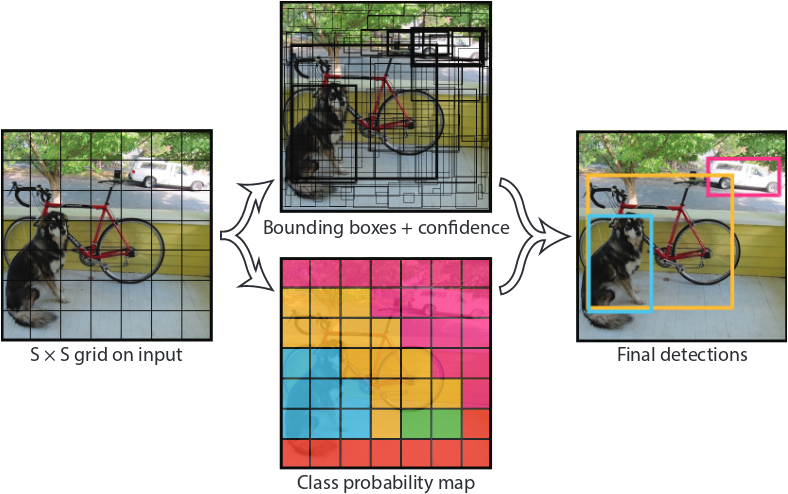
\includegraphics[width=0.8\textwidth]{Figs/Techanal/yolomodel.png}
      \caption{PLACEHOLDER. \gls{yolo} model.}
    \label{fig:yolomodel}
\end{figure}

As mentioned region proposals are found using the \gls{rpn} from Faster R-CNN \cite{fasterrcnn}. However, instead of using hand-picked priors for the anchor boxes, YOLOv2 proposed a method to learn more suitable sizes and aspect ratios. This is done by running k-means clustering on the annotated bounding boxes from the training set using a custom distance measurement. The custom measurement replaces Euclidean distance as these distances would create a bias due to more error on likely occurring on larger anchors. The custom distance measurement is designed for favourable \gls{iou} scores and is as follows:

\begin{equation}
  d(box, centroid) = 1 - IoU(box, centroid)
\end{equation}

where $box$ is the ground truth bounding box from the training set and $centroid$ is the predicted anchor box. By learning the priors YOLOv2 is able to use five anchor boxes at the same level of recall as the nine used in a typical \gls{rpn}.

YOLOv2 also goes against the grain in comparison to other state-of-the-art object detectors in regards to the choice of classification model. Rather than using the common networks such as VGG or ResNets, YOLOv2 propose their own 19 layer model dubbed Darknet-19. The model is of similar paradigm to VGG nets in that it uses mostly $3 \times 3$ convolutions and doubles the number of channels after pooling, which is also present in ResNets. But it is of considerably lower complexity than VGG-16 which consists of 15.3 billion \gls{flops}, with only 5.58 billion \gls{flops}. The baseline model has competitive results on ImageNet which can be seen in \tableref{darknetimagenet}. The baseline can be improved using standard data augmentations and also by initially training on $224 \times 224$ images followed by fine-tuning on $448 \time 448$, this is also shown as Darknet-19++ in \tableref{darknetimagenet}.

\begin{table}[h]
\centering
\caption{\gls{ilsvrc} classification results for the Darknet-19 model.}
\label{tab:darknetimagenet}
\begin{tabular}{|l|l|l|}
\hline
Model                                                                                       & top-1 error (\%) & top-5 error (\%) \\ \hline
Darknet-19                                                                                  & 27.1             & 8.8              \\ \hline
Darknet-19++ & 23.5             & 6.7              \\ \hline
\end{tabular}
\end{table}

To aid in the detection of small objects the Darknet-19 model is also pre-trained on high-resolution images from ImageNet prior to training for object detection. Also fine-grained features are passthrough from an earlier layer when performing prediction. This gives features from a $26 \times 26$ feature map instead of the $13 \time 13$ size at the \gls{rpn}. Finally multi-scale training is also performed.

\subsection{Benchmark Results}\label{sec:benchresults}
\begin{comment}
	RFCN
		train data union of voc 2007 trainval and voc 2012 trainval (07+12)
		test voc 2007 test set
		conv model ResNet-101
		slightly better on voc2007 (table 3)
		slight worse than Faster+++ (winner 2015) (table4)
			more bells/whistles
			rfcn only multiscale training
				train on coco - finetune on pascal
		faster
		depth - saturated at 101

    \subsection{Object Detection with ResNets}
    ResNets generalise well to computer vision tasks other than classification, such as object detection. The winning entries in 2015 from the authors of \cite{deepres} in \gls{ilsvrc} and \gls{mscoco} challenges for ImageNet detection, ImageNet localisation, COCO detection and COCO segmentation, were based upon the faster R-CNN framework with ResNets.
\end{comment}
This section will outline the results of the aforementioned \gls{cnn}-based object detectors on leading benchmarks \gls{pascalvoc} and \gls{mscoco}. This includes results on the methods with different combinations of \gls{cnn} models, training data, and additions such as multi-scale training. All results are taken from the respective authors papers.

\subsubsection{\gls{pascalvoc}}
A summary of the results on the test set of \gls{pascalvoc} 2007 can be seen in \tableref{07res}. The first column denotes which method is used while also stating the underlying \gls{cnn} model, for example VGG-16 or ResNet-101. Improvements to some of the baseline methods are also included in the first column if relevant. The improvements are online hard example mining (OHEM), multi-scale training (MSTR), multi-scale testing (MSTE), box refinement (BR), and global context (GC). Training data used in the various methods include the train set of \gls{pascalvoc} 2007 (07), train set of \gls{pascalvoc} 2012 (12), and trainval set from \gls{mscoco} (COCO). In entries when COCO is included, the detector is first trained on COCO followed by fine-tuning on 07+12. The best \gls{map} result for each combination of training data is shown in bold.


\begin{table}[h]
\centering
\caption{PASCAL VOC 2007 results.}
\label{tab:07res}
\begin{tabular}{|l|l|l|}
\hline
\textbf{method}                                                                   & \begin{tabular}[c]{@{}l@{}}\textbf{training} \\ \textbf{data}\end{tabular} & \textbf{mAP (\%)} \\ \hline
\begin{tabular}[c]{@{}l@{}}Faster R-CNN\\ VGG-16 \cite{fasterrcnn}\end{tabular}            & 07                                                       & 69.9     \\ \hline
\begin{tabular}[c]{@{}l@{}}Faster R-CNN\\ VGG-16 \cite{fasterrcnn}\end{tabular}            & 07+12                                                    & 73.2     \\ \hline
\begin{tabular}[c]{@{}l@{}}Faster R-CNN\\ ResNet-101 \cite{deepres}\end{tabular}        & 07+12                                                    & 76.4     \\ \hline
\begin{tabular}[c]{@{}l@{}}Faster R-CNN\\ ResNet-101\\ OHEM \cite{deepres}\end{tabular} & 07+12                                                    & 79.3     \\ \hline
\begin{tabular}[c]{@{}l@{}}R-FCN\\ ResNet-101 \cite{rfcn}\end{tabular}               & 07+12                                                    & 76.6     \\ \hline
\begin{tabular}[c]{@{}l@{}}R-FCN\\ ResNet-101 OHEM \cite{rfcn}\end{tabular}        & 07+12                                                    & 79.5     \\ \hline
\begin{tabular}[c]{@{}l@{}}R-FCN\\ ResNet-101 OHEM/MSTR \cite{rfcn}\end{tabular}      & 07+12                                                    & \textbf{80.5}     \\ \hline
\begin{tabular}[c]{@{}l@{}}YOLOv2 $288 \times 288$\\ DarkNet-19 \cite{yolov2}\end{tabular}                & 07+12                                                    & 69.0     \\ \hline
\begin{tabular}[c]{@{}l@{}}YOLOv2 $544 \times 544$\\ DarkNet-19 \cite{yolov2}\end{tabular}                & 07+12                                                    & 78.6     \\ \hline
\begin{tabular}[c]{@{}l@{}}Faster R-CNN\\ ResNet-101 BR/GC/MSTE \cite{deepres}\end{tabular}    & COCO+07+12                                               & \textbf{85.6}     \\ \hline
\begin{tabular}[c]{@{}l@{}}R-FCN\\ ResNet-101 OHEM/MSTR \cite{rfcn}\end{tabular}      & COCO+07+12                                               & 83.6     \\ \hline
\end{tabular}
\end{table}

A clear initial improvement is the use of ResNet-101 in comparison to the VGG-16 network, both with Faster R-CNN and \gls{rfcn}. ResNet-101 gives a \gls{map} improvement of 3.2\% in this scenario, from 73.2\% to 76.4\%. This was improvement was clear to the authors of \gls{rfcn} and therefore the only network used in their work is ResNet-101 for object detection. A small improvement of 0.2\% can also been seen for \gls{rfcn} over Faster R-CNN when using ResNet-101, both with and without \gls{ohem}. The best performing detector with 07+12 training data is \gls{rfcn} with both \gls{ohem} and MSTR (80.5\%), indicating that the addition of multi-scale training improves the result by 1\%. YOLOv2 scores slightly lower that \gls{rfcn} and Faster R-CNN. The best performing YOLOv2 network is trained to inputs of resolution $544 \times 544$, resulting in a \gls{map} of 78.6.
When using the method of training on COCO followed by fine-tuning on 07+12, Faster R-CNN with ResNet-101 and BR/GC/MSTE scoring 85.6\%. However, it is difficult to directly compare methods in this instance as the other method that uses the same training data, \gls{rfcn} with ResNet-101 and OHEM/MSTR, uses different variants of additions to the overall method. However, a general trend is that the training scheme of COCO+07+12 results in a significant improvement, with the comparable \gls{rfcn} method improving 3.1\%.

Similar results can be seen on the \gls{pascalvoc} 2012 testing set, shown in \tableref{12res}. A general standard for training on this test set is to include both the trainval and test from \gls{pascalvoc} 2007 and 2012 trainval, denoted as 07++12. As in the 2007 test set, Faster R-CNN is improved with the deeper features from ResNet-101 by 3.4\% when training with 07++12. The best result using the training set of 07++12 is with \gls{rfcn} with OHEM/MSTR, improving upon Faster R-CNN with ResNet-101 by 3.8\%. However, again it is difficult to compare due to the additions of OHEM and MSTR. The high-resolution version of YOLOv2 is again a number of percentage points behind resulting in 73.4\%. The best result is again of Faster R-CNN with ResNet-101 and BR/GC/MSTE when using COCO+07++12 as the training data with 83.8\%. \gls{rfcn} with ResNet-101 and OHEM/MSTR is similarly behind as in the 2007 test, scoring 1.8\% lower.


\begin{table}[h]
\centering
\caption{PASCAL VOC 2012 results.}
\label{tab:12res}
\begin{tabular}{|l|l|l|}
\hline
\textbf{method}                                                                  & \begin{tabular}[c]{@{}l@{}}\textbf{training} \\ \textbf{data}\end{tabular} & \textbf{mAP (\%)} \\ \hline
\begin{tabular}[c]{@{}l@{}}Faster R-CNN\\ VGG-16 \cite{fasterrcnn}\end{tabular}           & 12                                                       & 67.0     \\ \hline
\begin{tabular}[c]{@{}l@{}}Faster R-CNN\\ VGG-16 \cite{fasterrcnn}\end{tabular}           & 07++12                                                   & 70.4     \\ \hline
\begin{tabular}[c]{@{}l@{}}Faster R-CNN\\ ResNet-101 \cite{deepres}\end{tabular}       & 07++12                                                   & 73.8     \\ \hline
\begin{tabular}[c]{@{}l@{}}R-FCN\\ ResNet-101 OHEM/MSTR \cite{rfcn}\end{tabular}            & 07++12                                                   & \textbf{77.6}     \\ \hline
\begin{tabular}[c]{@{}l@{}}YOLOv2 $544 \times 544$\\ DarkNet-19 \cite{yolov2}\end{tabular} & 07++12                                                   & 73.4     \\ \hline 
\begin{tabular}[c]{@{}l@{}}Faster R-CNN\\ VGG-16 \cite{fasterrcnn}\end{tabular}           & COCO+07++12                                              & 75.9     \\ \hline
\begin{tabular}[c]{@{}l@{}}Faster R-CNN\\ ResNet-101 BR/GC/MSTE \cite{deepres}\end{tabular}       & COCO+07++12                                              & \textbf{83.8}     \\ \hline
\begin{tabular}[c]{@{}l@{}}R-FCN\\ ResNet-101 OHEM/MSTR \cite{rfcn}\end{tabular}            & COCO+07++12                                              & 82.0     \\ \hline
\end{tabular}
\end{table}

\subsubsection{\gls{mscoco}}
The final benchmark dataset to be compared is \gls{mscoco}. The results for this benchmark is more comprehensive than that shown in the \gls{pascalvoc} challenge. \gls{map} is calculated across a number of different \glspl{iou}. Also ground truths are split into three difference categories depending on the size of the object, denoted as either small, medium, or large. Training and testing data is done in two separate ways. Firstly, training is done on the train set of \gls{mscoco}, followed by testing on the validation set val. Secondly, training can be done on a combination of the aforementioned train and val (trainval), followed by testing on the test-dev set. The main results for the object detectors can be seen in \tableref{cocores}. A final testing set is also used for the YOLOv2 method, denoted trainval35k. Which is made up of the same images in trainval, however, 5,000 are removed for other validation purposes.

\begin{table}[h]
\centering
\caption{MS COCO test-dev results.}
\label{tab:cocores}
\begin{tabular}{|l|l|l|l|l|l|l|l|}
\hline
\textbf{method}                                                                 & \begin{tabular}[c]{@{}l@{}}\textbf{training}  \\ \textbf{data}\end{tabular} & \begin{tabular}[c]{@{}l@{}}\textbf{test}  \\ \textbf{data}\end{tabular} & \begin{tabular}[c]{@{}l@{}}\textbf{AP}\\ \textbf{@.5}\end{tabular} & \begin{tabular}[c]{@{}l@{}}\textbf{AP} \\ \textbf{@ [.5, .95]} \end{tabular} & \begin{tabular}[c]{@{}l@{}}\textbf{AP} \\ \textbf{small}\end{tabular} & \begin{tabular}[c]{@{}l@{}}\textbf{AP}  \\ \textbf{medium} \end{tabular} & \begin{tabular}[c]{@{}l@{}}\textbf{AP} \\ \textbf{large}\end{tabular} \\ \hline
\begin{tabular}[c]{@{}l@{}}Faster R-CNN\\ VGG-16 \cite{fasterrcnn}\end{tabular}          & train                                                    & val                                                  & 41.5                                              & 21.2                                                   & -                                                   & -                                                    & -                                                   \\ \hline
\begin{tabular}[c]{@{}l@{}}Faster R-CNN \\ ResNet-101 \cite{deepres}\end{tabular}     & train                                                    & val                                                  & 48.4                                              & 27.2                                                   & 6.6                                                 & 28.6                                                 & \textbf{45.0}                                                \\ \hline
\begin{tabular}[c]{@{}l@{}}R-FCN \\ ResNet-101 \cite{rfcn}\end{tabular}            & train                                                    & val                                                  & 48.9                                              & 27.6                                                   & \textbf{8.9}                                                 & 30.5                                                 & 42.0                                                \\ \hline
\begin{tabular}[c]{@{}l@{}}R-FCN \\ ResNet-101 \\ MSTR \cite{rfcn}\end{tabular}          & train                                                    & val                                                  & \textbf{49.1}                                              & \textbf{27.8}                                                   & 8.8                                                 & \textbf{30.8}                                                 & 42.2                                                \\ \hline
\begin{tabular}[c]{@{}l@{}}Faster R-CNN \\ VGG-16 \cite{fasterrcnn}\end{tabular}         & trainval                                                 & test-dev                                             & 42.7                                              & 21.9                                                   & -                                                   & -                                                    & -                                                   \\ \hline
\begin{tabular}[c]{@{}l@{}}Faster R-CNN \\ ResNet-101 \\ BR/GC/MSTE \cite{deepres}\end{tabular} & trainval                                                 & test-dev                                             & \textbf{55.7}                                              & \textbf{34.9}                                                   & \textbf{15.6}                                                & \textbf{38.7}                                                 & \textbf{50.9}                                                \\ \hline
\begin{tabular}[c]{@{}l@{}}R-FCN \\ ResNet-101 \cite{rfcn}\end{tabular}            & trainval                                                 & test-dev                                             & 51.5                                              & 29.2                                                   & 10.3                                                & 32.4                                                 & 43.4                                                \\ \hline
\begin{tabular}[c]{@{}l@{}}R-FCN \\ ResNet-101 \\ MSTR \cite{rfcn}\end{tabular}          & trainval                                                 & test-dev                                             & 51.9                                              & 29.9                                                   & 10.8                                                & 32.8                                                 & 45.0                                                \\ \hline
\begin{tabular}[c]{@{}l@{}}R-FCN \\ ResNet-101 \\ MSTR/MSTE \cite{rfcn}\end{tabular}         & trainval                                                 & test-dev                                             & 53.2                                              & 31.5                                                   & 14.3                                                & 35.5                                                 & 44.2                                                \\ \hline
\begin{tabular}[c]{@{}l@{}}YOLOv2\\ DarkNet-19 \cite{yolov2}\end{tabular}            & trainval35k                                              & test-dev                                             & 44.0                                              & 21.6                                                   & 5.0                                                 & 22.4                                                 & 35.5                                                \\ \hline
\end{tabular}
\end{table}

As in the \gls{pascalvoc} challenges, baseline \gls{rfcn} performs better than Faster R-CNN with ResNet-101, with \gls{ap}@.5 scoring 0.5\% and \gls{ap}@[.5, .95] 0.4\% higher. \gls{rfcn} with MSTR gives the best result when using the training set of \gls{mscoco} only. Interestingly this best result is not consistent when comparing \gls{ap} across the three object scales. For small object \gls{rfcn} with ResNet-101 is best at 8.9\%, slightly above \gls{rfcn} with ResNet-101 and MSTR (8.8\%). However, the later method is best for medium sized objects at 30.8\%, 0.3\% better than the next best method. Faster R-CNN with ResNet-101 performs best for large objects with 45.0\%, 2.8\% higher than the next best result, despite being considerably worse performing in the small and medium sized objects. When using the trainval set for training and test-dev for testing the best performing method is again Faster R-CNN with ResNet-101 and BR/GC/MSTE across all \gls{ap} modes. Again comparison is difficult as the methods do not all have the same additions to their baselines. \gls{rfcn} with ResNet-101 and MSTR/MSTE is competitive to the best result. According to the authors of the best method \cite{deepres}, the additions of box refinement gives roughly 2\% improvement, while global context gives about 1\%. This could account for the 2.5\% difference in \gls{ap}@.5. Finally YOLOv2 with DarkNet-19 performs considerably worse on \gls{mscoco}. This is especially present on smaller objects scoring 5.0\% \gls{ap}.